\documentclass[11pt]{article}
\usepackage[a4paper,margin=2.4cm]{geometry}
\usepackage[T1]{fontenc}
\usepackage{lmodern}
\usepackage{microtype}
\usepackage{amsmath}
\usepackage{graphicx}
\usepackage{booktabs}
\usepackage[numbers,sort&compress]{natbib}
\usepackage{xcolor}
\usepackage[colorlinks=true,linkcolor=blue!50!black,citecolor=blue!50!black,urlcolor=blue!50!black]{hyperref}
\usepackage{caption}
\captionsetup{font=small,labelfont=bf}
\graphicspath{{../figures/}}

\newcommand{\Rsq}{$R^2$}

\title{Remembering a Ball You Cannot See:\\Shortcuts, Memory and Attention in Occluded Pong}
\author{Giulio Sighieri\\\small Bocconi University, Deep Learning for Computer Vision}
\date{}

\begin{document}
\maketitle

\begin{abstract}
Agents trained on Pong have been found to rely on the opponent's paddle, which follows the ball, rather than
on the ball. We hide the ball in the agent's half of the court (fog), the opponent's paddle (mask), or both,
and ask whether agents then learn to remember a ball they cannot see, and how hard that is to learn. We train
three PPO agents of similar size that differ mainly in how they carry information over time: a CNN on four
stacked frames, a CNN with an LSTM, and a CNN whose LSTM reads the frame through attention steered by its own
memory, and test them with interventions on what they see, remember and attend to. Under fog with the
opponent's paddle visible, every agent depends on that paddle: erasing it costs almost every point. With
both hidden, the LSTM holds the hidden ball in its memory and acts on it: wiping the memory as the ball
disappears cuts the share of balls it returns from 0.98 to 0.30. The attention agent's memory depends on its
attention: in two of its four winning models, blocking attention to the ball before the fog makes it miss
most balls, while removing as much attention elsewhere costs nothing. The memoryless CNN wins without
tracking the incoming ball: it returns 0.80--0.94 of the balls with that ball erased from its view, because
rallies against the built-in opponent are regular enough to predict where the ball comes back after its own
shot. The attention agent learns the fog + hidden paddle view from scratch with one seed of three, and with
all three after pre-training on the clean game.
\end{abstract}

\section{Introduction}

Pong was among the first Atari games solved from pixels by deep reinforcement learning
\citep{mnih2013playing,mnih2015human}, and it remains a common first test for a new agent. Winning it,
however, does not mean the agent has understood it. \citet{delfosse2024scobots} found that agents trained on
Pong track the opponent's paddle rather than the ball. The built-in opponent follows the ball closely, so
its height is a good proxy for the ball's. HackAtari \citep{delfosse2024hackatari} confirmed the diagnosis:
when the opponent stops moving, the agents fall apart. This is shortcut learning \citep{geirhos2020shortcut}:
a cue that works on the training distribution replaces the one the task is about.

We use this to build a controlled test of memory. A \emph{fog} hides the ball in the agent's half of the
court, so the ball vanishes on its way towards the agent and reappears only at its paddle. A \emph{mask}
hides the opponent's paddle. With both, the agent cannot see the ball when it matters, nor anything that
tracks it. We ask two questions. \emph{Do agents learn to remember a ball they can no longer see, using the
tools their architecture gives them?} And \emph{how hard is that memory to learn?}

We compare three agents of similar size that differ mainly in how they carry information over time: a
\textbf{CNN} on four stacked frames, the DQN setup; an \textbf{LSTM} agent, which sees one frame per step
and keeps a recurrent memory \citep{hausknecht2015drqn}; and an \textbf{attention} agent, a simplified
version of \citet{mott2019attention}, whose memory decides where on the frame its attention looks. We
train each on the four combinations of fog and mask and test them with interventions rather than
correlations.

\paragraph{Findings.}
\begin{enumerate}
  \item \textbf{Under fog, the opponent's paddle remains the main cue.} With only the ball hidden, every
    agent depends on the opponent's paddle: erasing or mirroring it costs almost every point, and moving it 8
    pixels up most balls. The memory agents use the ball too: erasing it while it is still visible costs
    most of them part of their returns. With the ball in full view, by contrast, the clean CNN ignores the
    opponent's paddle entirely.
  \item \textbf{With nothing else to go on, the LSTM remembers the ball.} A linear probe reads the hidden
    ball's height from its memory (\Rsq{} 0.87--0.97, against 0.38--0.58 for an untrained LSTM), and wiping
    that memory as the ball disappears cuts the share of balls returned from 0.98 to 0.30.
  \item \textbf{The attention agent's memory depends on its attention.} Blocking attention to the ball
    before the fog makes the memory probe lose the ball in the three winning models whose heads track it;
    in two of them the agent then misses most balls, while removing as much attention elsewhere costs
    nothing.
  \item \textbf{The CNN predicts where the ball comes back.} On fog + hidden paddle it returns 0.80--0.94 of
    the balls with the incoming ball erased from its view (0.85--0.97 without), but loses whole games
    played without ever seeing the ball: it predicts the ball's return from its own last shot.
  \item \textbf{The attention agent's memory is hard to learn from scratch.} It learns fog + hidden paddle
    with one seed of three, and with all three after 10M steps on the clean game and 5M on fog + hidden
    paddle.
\end{enumerate}
Throughout, only interventions separate what an agent uses from what merely correlates with its behaviour:
natural attention, decodability and early movement each turn out to be poor guides on their own.

\section{Setup}

\begin{figure}[t]
  \centering
  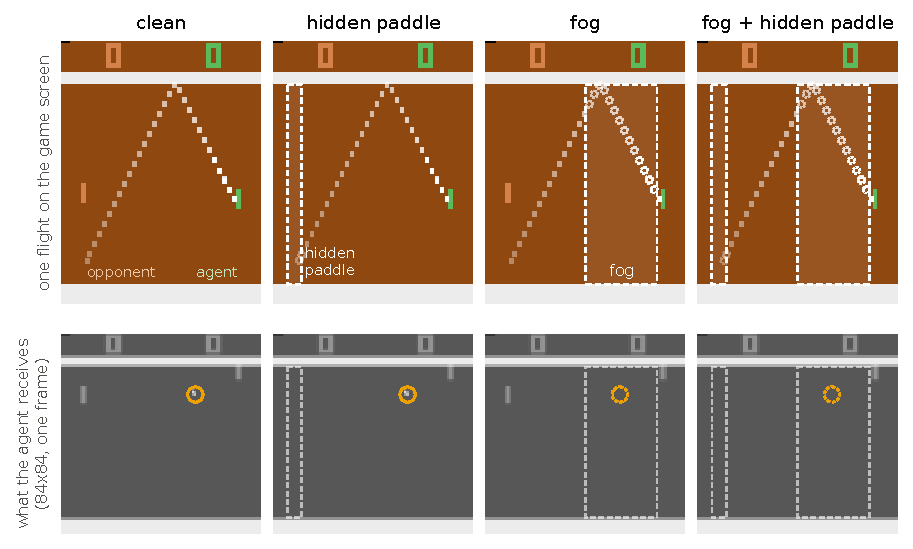
\includegraphics[width=\linewidth]{environments}
  \caption{The four views of Pong, on the game screen. One ball flight goes from the opponent's paddle (left)
    to the agent's (right), bouncing off the top wall. The path is solid where the agent's view shows the
    ball and dashed where it hides it. The fog covers the agent's half of the court (shaded here); in the
    agent's own $84\times84$ grayscale frame it is painted in the court's colour, so the ball simply vanishes
    there. The mask paints over the opponent's paddle (dashed outline). The agent always sees its own
    paddle.}
  \label{fig:views}
\end{figure}

\paragraph{Environment.} We use ALE Pong \citep{bellemare2013ale} through Gymnasium with the standard
preprocessing \citep{machado2018revisiting}: $84\times84$ grayscale frames, frame skip 4 (one agent step is
four emulator frames), up to 30 no-op starts, and no sticky actions. The occlusions are applied to the
observation only, so the game itself is unchanged. Figure~\ref{fig:views} shows the four views:
\textbf{clean}, \textbf{hidden paddle} (mask), \textbf{fog} (columns 42--71 of the frame), and \textbf{fog +
hidden paddle}. Under fog an incoming ball is invisible for about 14 agent steps; we call the step it
disappears \emph{fog entry}. For analysis, object positions are read from the unoccluded frame, which the
agent never sees.

\paragraph{Agents.} All agents share the Nature-CNN convolutions (three convolutional layers;
\citep{mnih2015human}) and separate linear actor and critic heads. They differ in what they keep from one
step to the next (Table~\ref{tab:agents}).
\begin{itemize}
  \item The \textbf{CNN} sees four stacked frames and maps them to 512 features. Its only memory is the stack.
  \item The \textbf{LSTM} agent sees one frame per step; its 512 features feed an LSTM with 128 units
    \citep{hochreiter1997lstm}.
  \item The \textbf{attention} agent also sees one frame. Its convolutions produce a $7\times7$ map of 64
    features, to which two fixed channels add each cell's $x$ and $y$ position. Each of eight heads scores
    the 49 cells with a query computed from the LSTM's previous hidden state $h_{t-1}$; the softmax-weighted
    sums of the cells' values (320 ReLU units per head) pass through a 512-unit ReLU layer into a 128-unit
    LSTM. This readout is the LSTM's only input, so what the agent remembers decides what it looks at next.
    We layer-normalise queries and keys without a learned scale; without this the attention stays uniform at
    initialisation and never learns where to look. The agent was widened to the LSTM agent's parameter count,
    so that differences between them are not a matter of size.
\end{itemize}

\begin{table}[t]
  \centering
  \small
  \begin{tabular}{llll}
    \toprule
    agent & input per step & memory & parameters \\
    \midrule
    CNN & 4 stacked frames & none (the stack) & 1.69M \\
    LSTM & 1 frame & LSTM, 128 units & 2.01M \\
    attention & 1 frame & LSTM, 128 units, fed by 8 attention heads & 1.98M \\
    \bottomrule
  \end{tabular}
  \caption{The three agents. All use the Nature-CNN convolutions and the same PPO hyperparameters.}
  \label{tab:agents}
\end{table}

\paragraph{Training.} PPO \citep{schulman2017ppo} follows CleanRL \citep{huang2022cleanrl}: 16 parallel
games, 256 steps per game per update, 4 epochs of 4 minibatches, $\gamma=0.99$, GAE $\lambda=0.95$, clip
0.1, entropy coefficient 0.02, and Adam with learning rate $10^{-3}$ annealed linearly to zero. The recurrent
agents are trained on whole 256-step sequences, with the memory reset at the end of each game. Every agent is
trained from scratch on every view for 15M agent steps, with three seeds. The attention agent is also trained
with a \emph{curriculum}: its clean model's 10M-step checkpoint is fine-tuned on each occluded view for 5M
steps, with a fresh optimiser and the learning rate restarted and annealed over those steps, for the same
15M total. As controls, the CNN and LSTM are fine-tuned from their clean models in the same way, for 5M and
for 15M steps.

\paragraph{Evaluation.} Each frozen model plays 30 games against the built-in opponent, with environment
seeds 10000--10029 and its stochastic policy. A game's return is points won minus points lost, from $-21$ to
$+21$; a model \emph{wins} a view if it wins most of its 30 games. The causal tests replay every ball flying
towards the agent from an exact emulator snapshot, in several branches that differ only by one intervention,
and compare the \emph{share of balls returned}: a ball counts as returned when the agent hits it back
across $x=40$ (the frame is 84 pixels wide), and each test replays up to 200 flights per model (600 for the
memory wipes). \emph{Erasing} an object paints its pixels in the court's colour in the frame the agent sees;
\emph{mirroring} the opponent's paddle draws it at the vertically opposite height. A model \emph{plays} a view if it returns at least half of
the balls without intervention; a model can return 80\% of the balls and still lose games, because the
opponent wins long rallies. A second unmodified replay, with different action noise, agrees with the first
within 0.04 everywhere.

\section{Results}

\subsection{What each agent learns}

\begin{figure}[t]
  \centering
  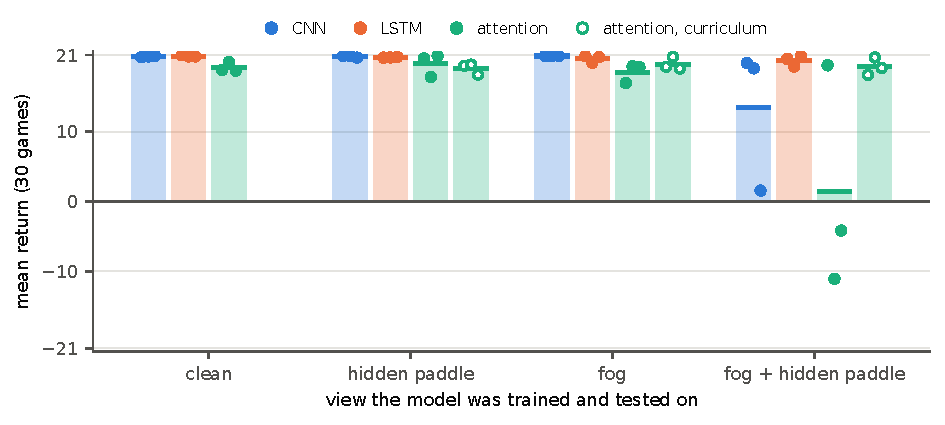
\includegraphics[width=\linewidth]{returns}
  \caption{Mean return of each final model on the view it was trained on (bars and ticks: mean over seeds;
    dots: seeds; 30 games each). Hollow: the attention agent's curriculum, pre-trained on the clean view for
    10M steps and fine-tuned on the target view for 5M (there is none for the clean view).}
  \label{fig:returns}
\end{figure}

Figure~\ref{fig:returns} shows how well each model plays its own view.
\begin{itemize}
  \item \textbf{Every agent learns the clean, hidden-paddle and fog views}, with every seed ($+17.0$ to
    $+20.9$), from scratch and with the curriculum.
  \item \textbf{Fog + hidden paddle separates them.} The LSTM agent wins with every seed ($+20.4$, $+19.3$,
    $+20.8$). The memoryless CNN wins with two ($+19.8$, $+19.1$, $+1.6$). The attention agent wins with one
    ($+19.5$, $-11.1$, $-4.2$), but with all three after the curriculum ($+18.1$ to $+20.6$).
\end{itemize}
Section~\ref{sec:learning} returns to how these models were learned. First we ask how they play.

\subsection{Under fog, every agent depends on the opponent's paddle}
\label{sec:shortcut}

\begin{figure}[t]
  \centering
  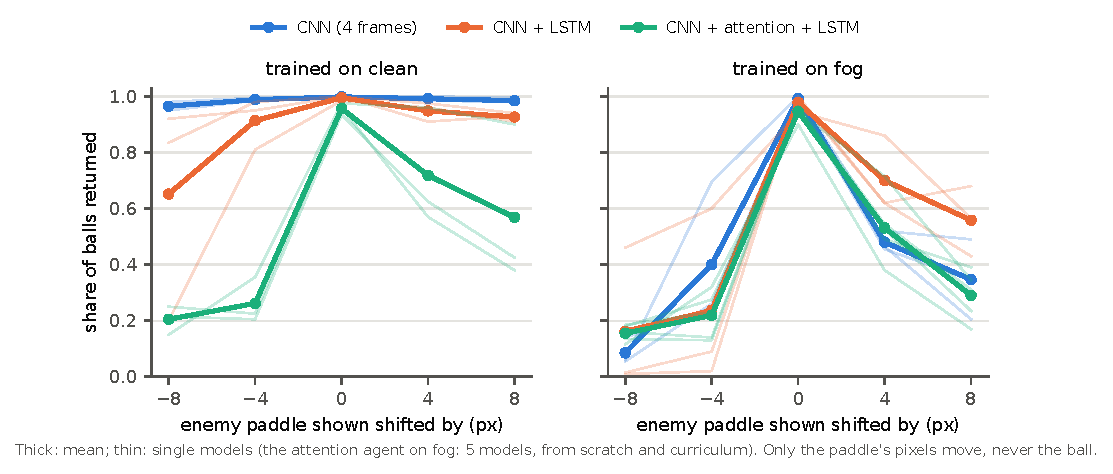
\includegraphics[width=0.9\linewidth]{shift}
  \caption{Share of balls returned when the opponent's paddle the model sees is moved by $-8$ to $+8$ pixels
    ($+$ is down). Only the paddle's pixels move; the ball and the game are unchanged. Thick lines: mean over
    models; thin lines: single models (the attention agent counts from scratch and with the curriculum).
    Models that do not play their view are left out. Left: models trained on the clean view. Right: models
    trained on fog.}
  \label{fig:shift}
\end{figure}

If the fog forced the agents to remember the ball, a fog-trained agent would not need the opponent's
paddle. But it still does.
\begin{itemize}
  \item \textbf{Erasing or mirroring the paddle} (flipping it to the opposite height) in what the agent sees
    makes every fog-trained model lose almost every point ($-20.2$ to $-21.0$), although the real ball
    still reaches its paddle.
  \item \textbf{A small shift is enough} (Figure~\ref{fig:shift}). Moving the paddle the agent sees 8
    pixels up cuts the share of balls returned from 0.90--1.00 to 0.01--0.46 in every fog model (three CNN,
    three LSTM and six attention models), and a 4-pixel upward shift removes over a third of it in 10 of
    the 12. Downward shifts cost less and less consistently (0.15--0.89 at 8 pixels). The clean CNN does not notice any shift (0.95 or more), so the effect is not a
    generic response to an edited frame.
  \item \textbf{Clean models differ by architecture.} With the paddle erased, the clean CNN still wins
    ($+20.0$ to $+20.7$): unlike the agents of \citet{delfosse2024scobots}, it ignores the opponent's paddle.
    The clean LSTM and attention models depend on it to varying degrees ($+18.8$, $-11.0$, $+7.5$ and
    $+15.7$, $-20.2$, $-4.6$). With the ball in full view, then, the shortcut is a matter of architecture
    and seed; under fog, where the paddle is a genuinely informative cue, every agent uses it.
  \item \textbf{The fog attention models look at it.} Inside the fog, one head of every fog model turns to
    the opponent's paddle (0.34--0.75 of its weight, against 0.06 for uniform attention;
    Figure~\ref{fig:attention}).
\end{itemize}
How the paddle is read remains open. The way the agents move their own paddle after a shift is not
consistent across models: some move against the shift, some move the same way whichever way it is shifted,
and some respond to one direction only. None simply follows the shifted paddle. An edited paddle may matter
most at the moment it hits the ball, which sets the ball's angle, rather than as a running height signal;
we have not separated the two.

The paddle is necessary, but not always sufficient. Erasing the ball while it is still visible, before the
fog, also costs seven of the nine fog-trained LSTM and attention models part of their returns (from
0.88--1.00 to 0.26--0.82). With the ball erased for the whole flight, the fog CNN still returns 0.92--0.98
of the balls from the paddle alone (and wins whole games played without the ball, $+5.0$ to $+18.1$), while
the LSTM returns 0.52--0.95 and the attention agent 0.20--0.94. Scripted players on the same games under fog put this in perspective:
copying the opponent's paddle returns 0.55 of the balls, going to the ball's last seen height 0.66, and
extrapolating its seen path 0.88 (0.96 without fog). The trained agents (0.90--1.00) combine both sources.

\subsection{With the shortcut gone, the LSTM remembers the ball}
\label{sec:lstm}

\begin{figure}[t]
  \centering
  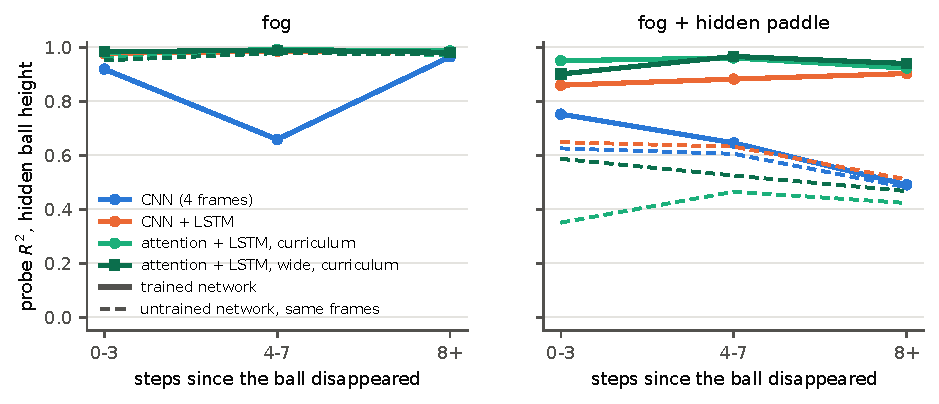
\includegraphics[width=0.8\linewidth]{probes}
  \caption{Held-out \Rsq{} of a linear probe for the hidden ball's height from each model's internal state
    (LSTM $[h,c]$; for the CNN, its 512 features), by steps since fog entry. Solid: the trained model.
    Dashed: an untrained network of the same architecture fed the same frames. The attention agent is shown
    with the curriculum, the only variant that wins fog + hidden paddle with every seed. On fog, the
    untrained networks decode the ball as well as the trained ones (the trained CNN dips at 4--7 steps,
    when the ball has just left its four-frame stack).}
  \label{fig:probes}
\end{figure}

\paragraph{Probes.} Following \citet{alain2016probes} and \citet{anand2019atariari}, we fit ridge
regressions, cross-validated over games, from each model's state to the ball's height while it is hidden.
To separate memory from input, every frame is also fed to an untrained network of the same architecture,
with its own memory, and probed the same way (Figure~\ref{fig:probes}).
\begin{itemize}
  \item \textbf{Under fog alone, decodability is not memory.} Eight or more steps in, the hidden ball decodes
    almost perfectly from every model and from the untrained networks (\Rsq{} 0.95--0.99), because the
    visible opponent paddle tracks it.
  \item \textbf{On fog + hidden paddle, only trained memory holds the ball.} Eight or more steps in, the
    LSTM's memory gives \Rsq{} 0.87--0.97 against 0.38--0.58 for the untrained LSTM, and the curriculum
    attention agent's 0.92--0.97 against 0.19--0.70. The CNN's features decode the ball no better than an
    untrained CNN's (0.40--0.57 against 0.39--0.55). Part of what the probe reads may be the agent's plan
    for where to meet the ball rather than the ball itself; the wipes below show that it is used.
\end{itemize}

\begin{figure}[t]
  \centering
  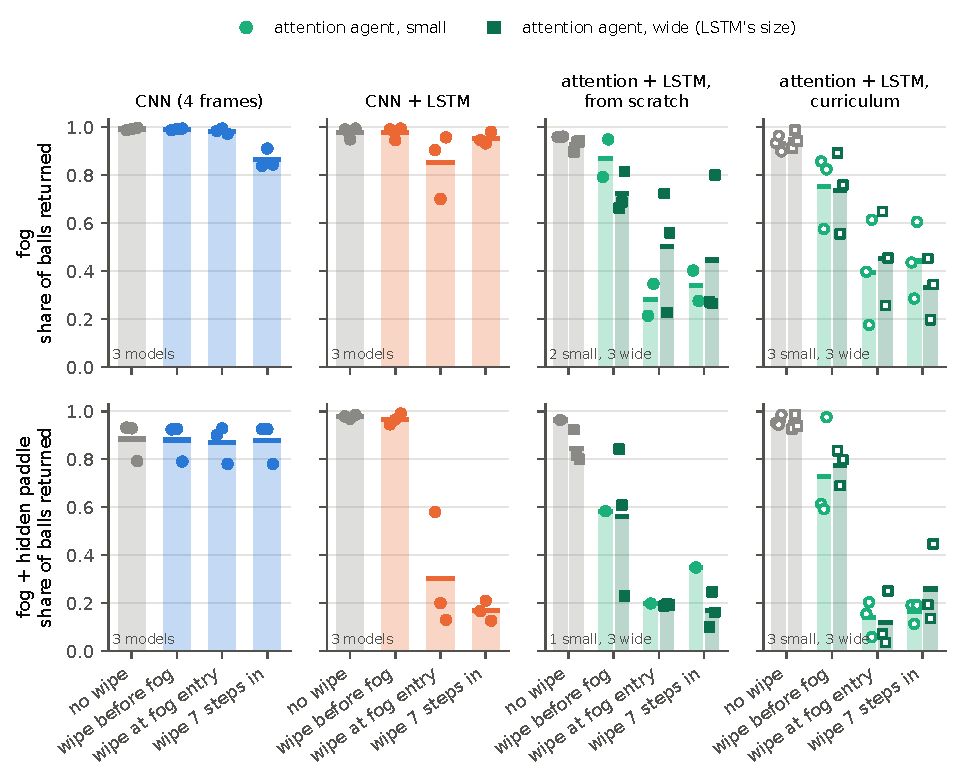
\includegraphics[width=0.85\linewidth]{wipes}
  \caption{Share of balls returned when the memory is wiped (LSTM state set to zero; for the CNN, the frame
    stack filled with the current frame for four steps) at one of three moments: while the ball is still
    visible (as it crosses $x=30$, a few steps before the fog); at fog entry; or seven steps after it. Rows: training view.
    Grey: no wipe. Bars and ticks: mean over models; dots: models; hollow: curriculum.}
  \label{fig:wipes}
\end{figure}

\paragraph{Memory wipes.} A probe shows that information is present; whether it is used is a separate
question. We therefore wipe
the memory and replay each ball (Figure~\ref{fig:wipes}).
\begin{itemize}
  \item \textbf{The fog + hidden paddle LSTM depends on its memory.} A wipe at fog entry drops the share of
    balls returned from 0.97--0.98 to 0.58, 0.20 and 0.13; seven steps in, to 0.13--0.21. A wipe before the
    fog costs nothing (0.94--0.99), because the ball is seen again.
  \item \textbf{The fog-only LSTM barely needs memory} (0.70--0.96 after a wipe at fog entry): with the
    opponent's paddle in view it rebuilds its estimate.
  \item \textbf{The CNN does not use its last views of the ball.} No wipe of its frame stack changes its
    share on fog + hidden paddle (0.78--0.93 in every branch; Section~\ref{sec:cnn}).
\end{itemize}

\paragraph{Timescale.} Recomputed on their own games, the forget gates of the fog + hidden paddle LSTMs
give their ten slowest units half-lives of 18.5, 16.5 and 8.3 steps, of the order of the 14 steps the ball
stays hidden, while clean LSTMs keep units that hardly forget.

\subsection{The attention agent remembers what its ball head lets in}
\label{sec:attention}

\begin{figure}[t]
  \centering
  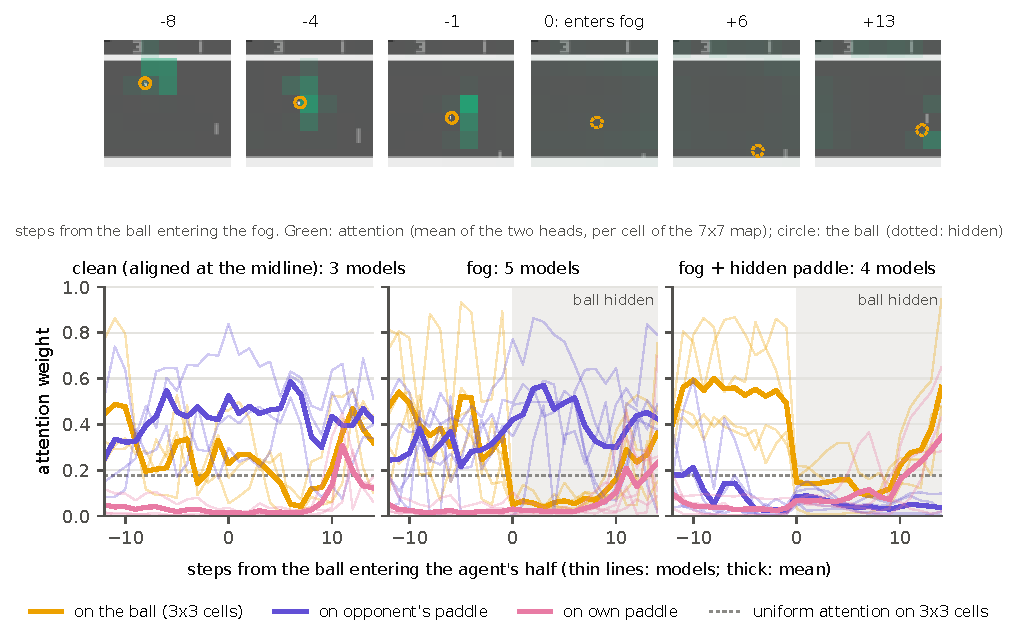
\includegraphics[width=\linewidth]{attention}
  \caption{Where the attention agent looks while a ball comes towards it. Top: one returned flight of a
    curriculum model on fog + hidden paddle, on the frames the agent sees, with the weights of its ball head
    (green; circle: the ball, dotted while hidden). Bottom: for every model that plays its view, the ball
    head's weight on the ball's $3\times3$ cells and the paddle head's weight on the opponent's paddle,
    aligned on fog entry (clean: on the ball crossing the midline). Each model's heads are chosen on half of
    its returned flights and plotted on the other half, so choosing the best of eight heads does not flatter
    them. On fog + hidden paddle the opponent's paddle is masked, so the paddle head's weight there is on an
    empty region. Dotted: uniform attention.}
  \label{fig:attention}
\end{figure}

\paragraph{Wipes.} The attention agent depends on its memory at least as much as the LSTM agent. On fog +
hidden paddle, a wipe at fog entry leaves 0.04--0.25 of the balls returned; even on fog, with the opponent's
paddle in view, it recovers less (0.23--0.72). Unlike the LSTM agent, it is also hurt by a wipe before the
fog (0.23--0.89), because its memory sets its attention: a wipe both erases what it remembers and disturbs
where it looks.

\paragraph{Where it looks.} Each of its eight heads is free to look anywhere; Figure~\ref{fig:attention}
follows, in each model, the head that looks most at the ball and the one that looks most at the opponent's
paddle. On fog + hidden paddle, in three of the four winning models a head follows the ball cell by cell
while it is visible (0.87--0.97 of its weight on the ball's cells in the eight steps before the fog, against
0.18 for uniform attention), lets it go in the first eight steps of the fog (0.02--0.26), and finds it
again as the ball reappears near the paddle. On fog, in every model a head turns
to the opponent's paddle inside the fog (Section~\ref{sec:shortcut}). Natural attention is a weak
guide on its own, however: per flight, attention to the ball before the fog does not predict the memory's
error inside it consistently across models (Spearman $-0.11$ to $+0.42$).

\paragraph{Blocking attention.}

\begin{figure}[t]
  \centering
  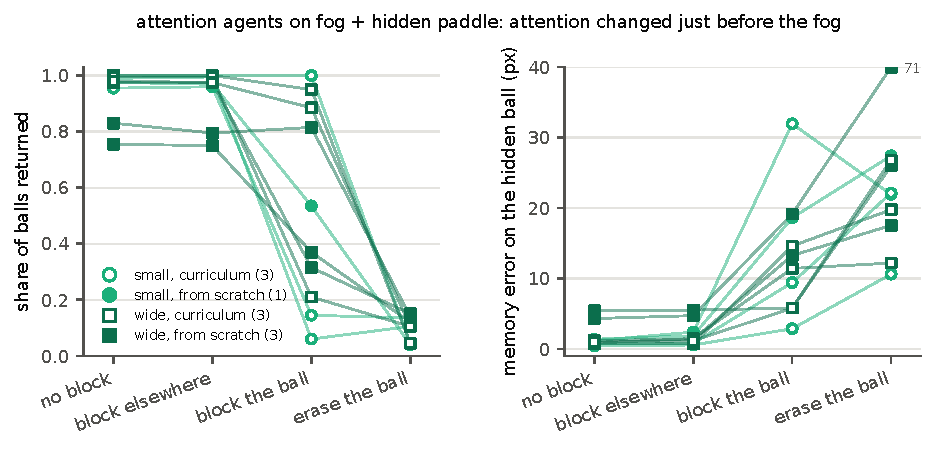
\includegraphics[width=0.9\linewidth]{block}
  \caption{The attention agent on fog + hidden paddle. Each incoming ball is replayed while, as long as the
    ball is visible before the fog, the agent may not attend to the $3\times3$ cells around it (\emph{block
    the ball}). The control blocks the cells with the most attention elsewhere until they hold as much
    attention as the ball's cells (\emph{block elsewhere}), and \emph{erase the ball} removes the ball from
    the screen. Left: share of balls returned. Right: mean absolute error of the memory probe on the hidden
    ball's height (one value of 71\,px drawn at the edge). Lines: models; hollow: curriculum. The two
    from-scratch models that do not win still return 0.76 and 0.83 of the balls unblocked.}
  \label{fig:block}
\end{figure}

The readout is the only path from the frame to the attention agent's memory, so we can ask directly whether
it remembers only what it attends to. While the ball is visible before the fog, we remove the $3\times3$ cells
around it from every head's softmax (their scores set to $-\infty$ before normalising); neither paddle's
cells are ever blocked. As a control, a second branch removes, at each step, the cells with the most
attention (averaged over heads) outside the ball and the paddles, until they hold at least as much attention
as the ball's cells; a third erases the ball from the screen (Figure~\ref{fig:block}). The control matches
the total attention removed; it does not match the disruption to each head: the ball head, which puts most of its weight on
the ball, is changed more by the ball block. Each model replays up to 200 flights from ten new games.
\begin{itemize}
  \item \textbf{Blocking the ball makes the memory probe lose it.} In the three winning models whose ball
    head tracks it, the probe's error on the hidden ball rises from about 1\,px to 11--15\,px. In two of them
    the agent then misses most balls (from 0.97 and 0.99 to 0.32 and 0.21).
  \item \textbf{The same attention removed elsewhere changes nothing} in those two models (0.95 and 0.99 of
    balls returned; probe error 1.9 and 0.8\,px), so the effect is specific to the ball rather than to disturbing the
    softmax.
  \item \textbf{Not every model gates the ball through one head.} In the third tracking model the probe
    loses the ball (11\,px) but the agent still returns 0.95 of the balls. In the winning model whose heads
    barely track the ball, blocking it costs little (0.89); blocking its most-attended cells elsewhere,
    which removes twice as much attention, costs more (0.76).
  \item \textbf{Models that are still learning are fragile.} In the two from-scratch models that do not
    win, either block disturbs play (0.76 to 0.37 and 0.53; 0.83 to 0.81 and 0.21), so they say little
    about the ball.
\end{itemize}

\subsection{The CNN predicts where the ball comes back}
\label{sec:cnn}

The CNN wins fog + hidden paddle with two seeds, yet no wipe of its frame stack changes anything
(Figure~\ref{fig:wipes}), and a probe reads no more of the hidden ball from its features than from an
untrained CNN's (Section~\ref{sec:lstm}). Its play looks like early commitment: in its two winning seeds,
four steps into the fog its paddle is already about 6\,px from where the ball will arrive (LSTM 11--43\,px,
winning attention models 12--17\,px), and it makes only 4--10\% of its movement in the last four steps.
Three interventions show what it relies on.
\begin{itemize}
  \item \textbf{Holding its paddle still} from the moment the ball leaves the opponent until four steps
    after fog entry, when its frame stack no longer shows the ball, barely changes the share of balls it
    returns (from 0.85--0.97 to 0.77--0.92). It does not need to move early.
  \item \textbf{Erasing the incoming ball} from every frame it sees, from the opponent's hit until the
    point ends, barely changes it either (0.80--0.94). The same erasure leaves the clean CNN 0.12 of the
    balls, and the fog + hidden paddle LSTM and attention agent 0.06--0.14.
  \item \textbf{Erasing the ball for whole games}, its own returns included, makes it lose every game
    ($-14.9$ to $-19.0$).
\end{itemize}
The CNN does not track the incoming ball; it predicts where the ball will come back from the rally it has
just seen. Against the built-in opponent this is a good bet: in the games of every model that wins fog +
hidden paddle, 74--95\% of the balls arrive within 4\,px of their usual height (in losing models' games,
11--56\%; we cannot tell cause from effect), and the CNN's paddle waits near that height (its spread at
arrival is 3--5\,px in the winning seeds). Rallies alone do not decide the strategy: the LSTM's and the
attention agent's are as regular, yet their play collapses without the incoming ball. They use what they
see and remember; the CNN, which cannot remember, uses the regularity. The fog + hidden paddle view can
therefore be won without carrying the ball through the fog, which qualifies it as a test of memory.

\subsection{Learning to remember}
\label{sec:learning}

\begin{figure}[t]
  \centering
  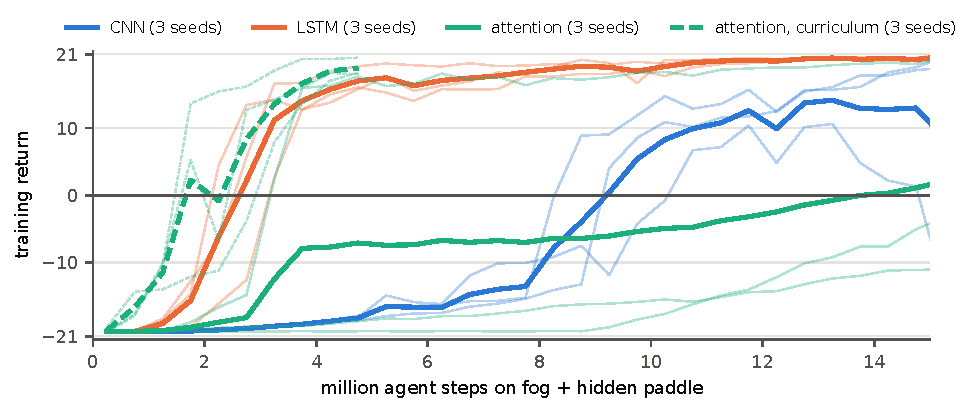
\includegraphics[width=\linewidth]{learning}
  \caption{Training return on fog + hidden paddle against steps played on that view (mean of the training
    games in each 0.5M-step bin). Thin: seeds; thick: mean. Dashed: the attention agent's curriculum, whose
    5M steps on this view follow 10M on the clean one.}
  \label{fig:learning}
\end{figure}

Figure~\ref{fig:learning} shows how the fog + hidden paddle models were learned.
\begin{itemize}
  \item \textbf{The LSTM agent learns quickly with every seed}: its training return turns positive within
    2.5--3.5M steps.
  \item \textbf{The attention agent learns as fast, or much more slowly.} Its one winning seed turns
    positive at 3.5M steps, as fast as the LSTM. The other two stay near $-20$ for 4M and 10M steps and are
    still improving when training stops at 15M ($-11$ and $-3$ in training). One of them (seed 2) was
    restarted from its 1M checkpoint with a fresh optimiser after a non-finite loss at 1.34M steps.
  \item \textbf{With the curriculum, every seed learns.} Fine-tuned from its clean model, every seed turns
    positive within 2--3.5M of the 5M steps (3 of 3, against 1 of 3 from scratch).
  \item \textbf{The CNN needs much longer}: two seeds turn positive after 9--9.5M steps; the third gets
    there at 11M and falls back. This fits a strategy that pays only once rallies have become regular
    (Section~\ref{sec:cnn}).
\end{itemize}
The curriculum differs from scratch training in two ways at once: the clean weights, and a fresh optimiser
with the learning rate restarted. We have not separated them. For the CNN and LSTM the same 5M-step
fine-tuning is not enough (their fine-tunes are still losing at 5M, $-15.5$ and $-8.9$ in evaluation), but
this comparison is confounded by the schedule, which anneals the learning rate to zero over 5M steps. Given
the full 15M with the scratch schedule, every CNN and LSTM fine-tune wins ($+13.3$ to $+20.9$), and two LSTM
fine-tunes learn faster than their scratch runs ($+9.1$ and $+13.8$ after 2M steps, against $-8.7$ and
$-8.2$). Clean pre-training is thus a good start for every agent, and for the attention agent it went with
winning in all three seeds. One explanation, which we have not tested, is a chicken-and-egg problem: the
attention agent's memory holds what its attention lets in, and its attention is steered by its memory. A
clean model already has heads that track the ball, and memory can build on them.

\section{Related work}

\citet{hausknecht2015drqn} replaced DQN's frame stack with an LSTM and showed that recurrence helps when frames
are randomly blanked (flickering Pong); recurrent model-free agents are strong baselines in partially
observable tasks \citep{ni2022recurrent}. Our occlusion is structured instead: one region, always hidden, so
that memory, a shortcut, or a prediction from the rally are all possible solutions, and we ask which one each
agent finds. Attention over a spatial feature map was added to recurrent Atari agents by DARQN
\citep{sorokin2015darqn} and made interpretable by \citet{mott2019attention}, whose design we simplify. That
attention weights need not explain a model's behaviour was argued for NLP \citep{jain2019attention}, and
saliency maps of Atari agents were found not to survive counterfactual tests \citep{atrey2020exploratory}; we
therefore intervene on attention rather than read it. Linear probes for Atari state follow AtariARI
\citep{anand2019atariari}, and our untrained-network baseline plays the role of a probe control
\citep{hewitt2019control}. Shortcut learning \citep{geirhos2020shortcut} was diagnosed for Pong by SCoBots
\citep{delfosse2024scobots} and HackAtari \citep{delfosse2024hackatari}, and policies that pursue a proxy of
their goal have been studied as goal misgeneralisation \citep{langosco2022goal}. Clean-then-hard training is a
simple curriculum \citep{bengio2009curriculum}.

\section{Limitations}

\begin{itemize}
  \item \textbf{Scale.} Three seeds per condition and a single game against a single opponent. The learning
    result rests on 1 of 3 seeds against 3 of 3 (Fisher's exact test, $p=0.4$), and several mechanistic
    findings on two to four models. Effects smaller than 0.04 in the share of balls returned are within the
    replay noise.
  \item \textbf{Interventions leave the training distribution.} An erased or mirrored paddle, a blocked
    attention cell, an erased ball and a wiped memory are all states the agents never saw in training. We
    pair each with a control (the clean CNN under the paddle edits, attention removed elsewhere, a wipe
    before the fog, the clean and memory agents under ball erasure), but a control cannot rule out every
    non-specific effect. The probes are fit on natural states, so their errors under an intervention are only
    indicative.
  \item \textbf{Shared hyperparameters.} Every agent uses the same PPO settings, including the learning rate
    of $10^{-3}$, which was not tuned per architecture and may favour some agents.
  \item \textbf{Evaluation} uses the stochastic policy against the built-in opponent only, whose regular
    rallies make the fog + hidden paddle view winnable without memory (Section~\ref{sec:cnn}).
  \item \textbf{Training history.} Some runs were resumed after interruptions: power cuts at the training
    machine (from the latest saved checkpoint; the 15M-step fine-tuning controls with a fresh optimiser, and
    the attention agent's hidden-paddle and fog curriculum runs restarted from their 10M starting point), and
    one non-finite loss (Section~\ref{sec:learning}). Every restart is recorded in the training logs.
\end{itemize}

\paragraph{Availability and compute.} Code, analysis scripts and the data behind every figure are in the
project repository (\url{https://github.com/WindyITS/ppo_atari}). Every model was trained on one NVIDIA RTX
3070 (8\,GB); a 15M-step run takes about 16 hours with six runs sharing the GPU.

\section{Conclusion}

With the opponent's paddle in view, every agent leans on it, even when a fog hides the ball in its own half.
Without it, the two recurrent agents carry the hidden ball in their memory and act on it, and the attention
agent's memory holds what its attention lets in. The memoryless CNN finds a third way: it predicts where the
ball will come back from the rally it has just seen, which the regular play of the built-in opponent allows.
The attention agent, whose memory and attention depend on each other, learned the hardest view reliably only
after the easier game. Throughout, it took interventions to tell these strategies apart.

\bibliographystyle{plainnat}
\bibliography{refs}

\end{document}
